\section{\name}
\label{sec:systemDesignMain}

Our goal is to design a solution that addresses the above limitations of previous solutions. In short, our solution should be \emph{secure} (no TOFU assumption, small TCB, no online authorities) and \emph{easy to deploy} (no OS re-installation, manual configuration, or pre-defined enclaves). In this section, we provide an overview of our approach, outline possible use cases, describe our solution in detail, and analyze its security.

\subsection{Approach Overview}

We propose a hardened SGX attestation scheme, called \name, based on a simple embedded device that we call \device. The embedded device is attached to the target platform over a local communication interface such as a USB. 

% as shown in  Figure~\ref{fig:approach}. %Using this approach, we propose a hardened attestation mechanism to address the relay attacker defined in Section~\ref{sec:problemStatement:attackerModel}.

Our main idea is to use the combination of such a trusted device and \emph{proximity verification} to prevent relay attacks. In our solution, the \device device verifies the proximity of the attested enclave, and after successful proximity verification, it facilitates the creation of a secure channel between the remote verifier and the attested enclave. 

After the initial attestation, the device periodically checks proximity to the attested enclave. The established secure channel is contingent on the physical presence of the embedded device on the target machine, and it stays active only as long as the device is plugged in. The act of detaching the device automatically revokes the attested platform without any interaction with a trusted authority. Thus, our solution enables secure \emph{offline} enrollment and revocation. 

To use our solution, enclave developers use a simple API that facilitates communications between the enclave and the device. 


\myparagraph{Security assumptions}
%\label{sec:ext-attacker-model}
In our solution, the \device device is a trusted component. We deem this choice reasonable since it implements only the strictly necessary functions, and therefore, it has significantly smaller software TCB, attack surface, and complexity compared to a general-purpose commodity OS. We assume that its issuer certifies each embedded device prior to its deployment, and such certification can take place fully offline.

Concerning the security of the \device device we employ the same attacker model introduced in Section~\ref{sec:problemStatement} for enclaves. While the user's device and its private keys are never exposed to the attacker, another similar device can be in the physical possession of the attacker, which has as much time as she wants to fully compromise it (run arbitrary code and extract keys). 


\subsection{Example Use Cases}
\label{sec:use-cases}

Our solution is targeted to scenarios where the benefits of more secure attestation outweigh the deployment cost of a simple embedded device. Here, we outline three example cases.  

\myparagraph{Data center} In our first example, we consider a cloud platform provider that attaches \device to a server in a specific data center and makes the public key of the connected device known to the users of the service. Our approach is particularly well suited to cloud computing models where customers rent dedicated computing resources like entire servers. In such a setting, our solution ensures that the cloud platform customer outsources data and computation to a server that resides in a specified location. Enforcing location may be desirable to meet increasing data protection regulation that defines how and where data can be stored, even if protected by TEEs such as SGX. Revocation (e.g., when a server is relocated to another data center or function) can be realized by merely detaching \device.

\myparagraph{Permissioned blockchain} Our second case is a setting in which a trusted authority initializes a set of validator nodes for a permissioned and SGX-hardened blockchain. 
The trusted authority issues one \device for each organization that operates one of the validator nodes, which allows secure attestation of the validator platforms. Organizations are free to upgrade their computing platforms by attaching the \device to a new platform which automatically revokes the old platform without the need to interact with a trusted authority. Furthermore, since \device can only be active on one platform at a time, such a deployment enables the authority to control the identities used in a (Byzantine) blockchain consensus process.



\myparagraph{HSM-protected keys} Our last case is the management of HSM-protected keys from an attested enclave. Such deployment enables the secure and flexible realization of various access control policies, implemented as attested enclaves. \name guarantees that only an enclave in the proximity of the HSM can control its keys. Such a solution provides a high level of protection because, at no point in time, the HSM keys are directly accessible by the enclave (which may be vulnerable to side-channel attacks) or by the untrusted OS.


\subsection{Solution Details}
\label{sec:systemDesign}


Now, we explain the \name attestation mechanism in detail.


\myparagraph{Attestation protocol} 

Figure~\ref{fig:systemSetUp} illustrates the attestation protocol that proceeds as follows:


\begin{figure}[t]
 \centering
  %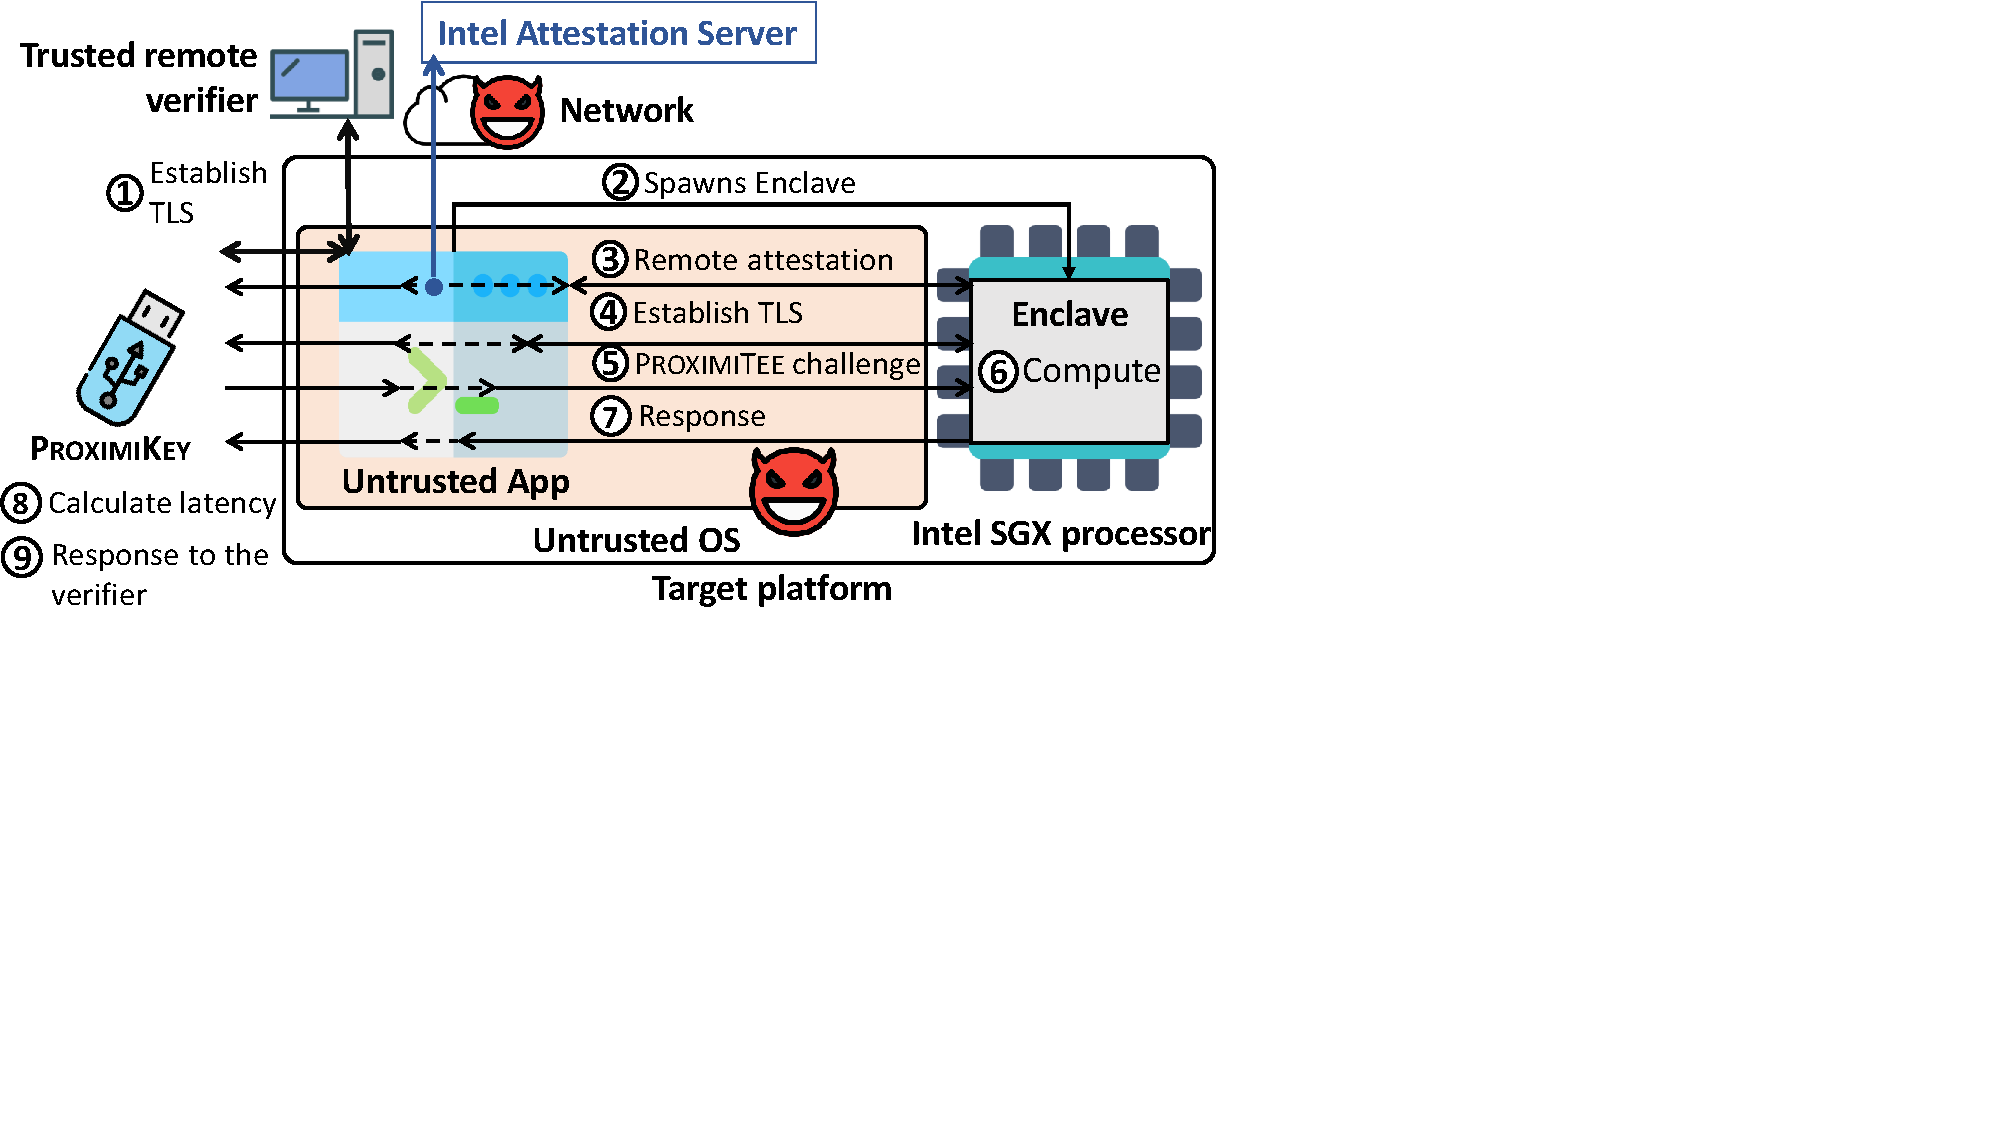
\includegraphics[trim={0 8.7cm 13.2cm 0},clip,width=\linewidth]{chapters/ProximiTEE/figures/proximiteeMain.pdf}
  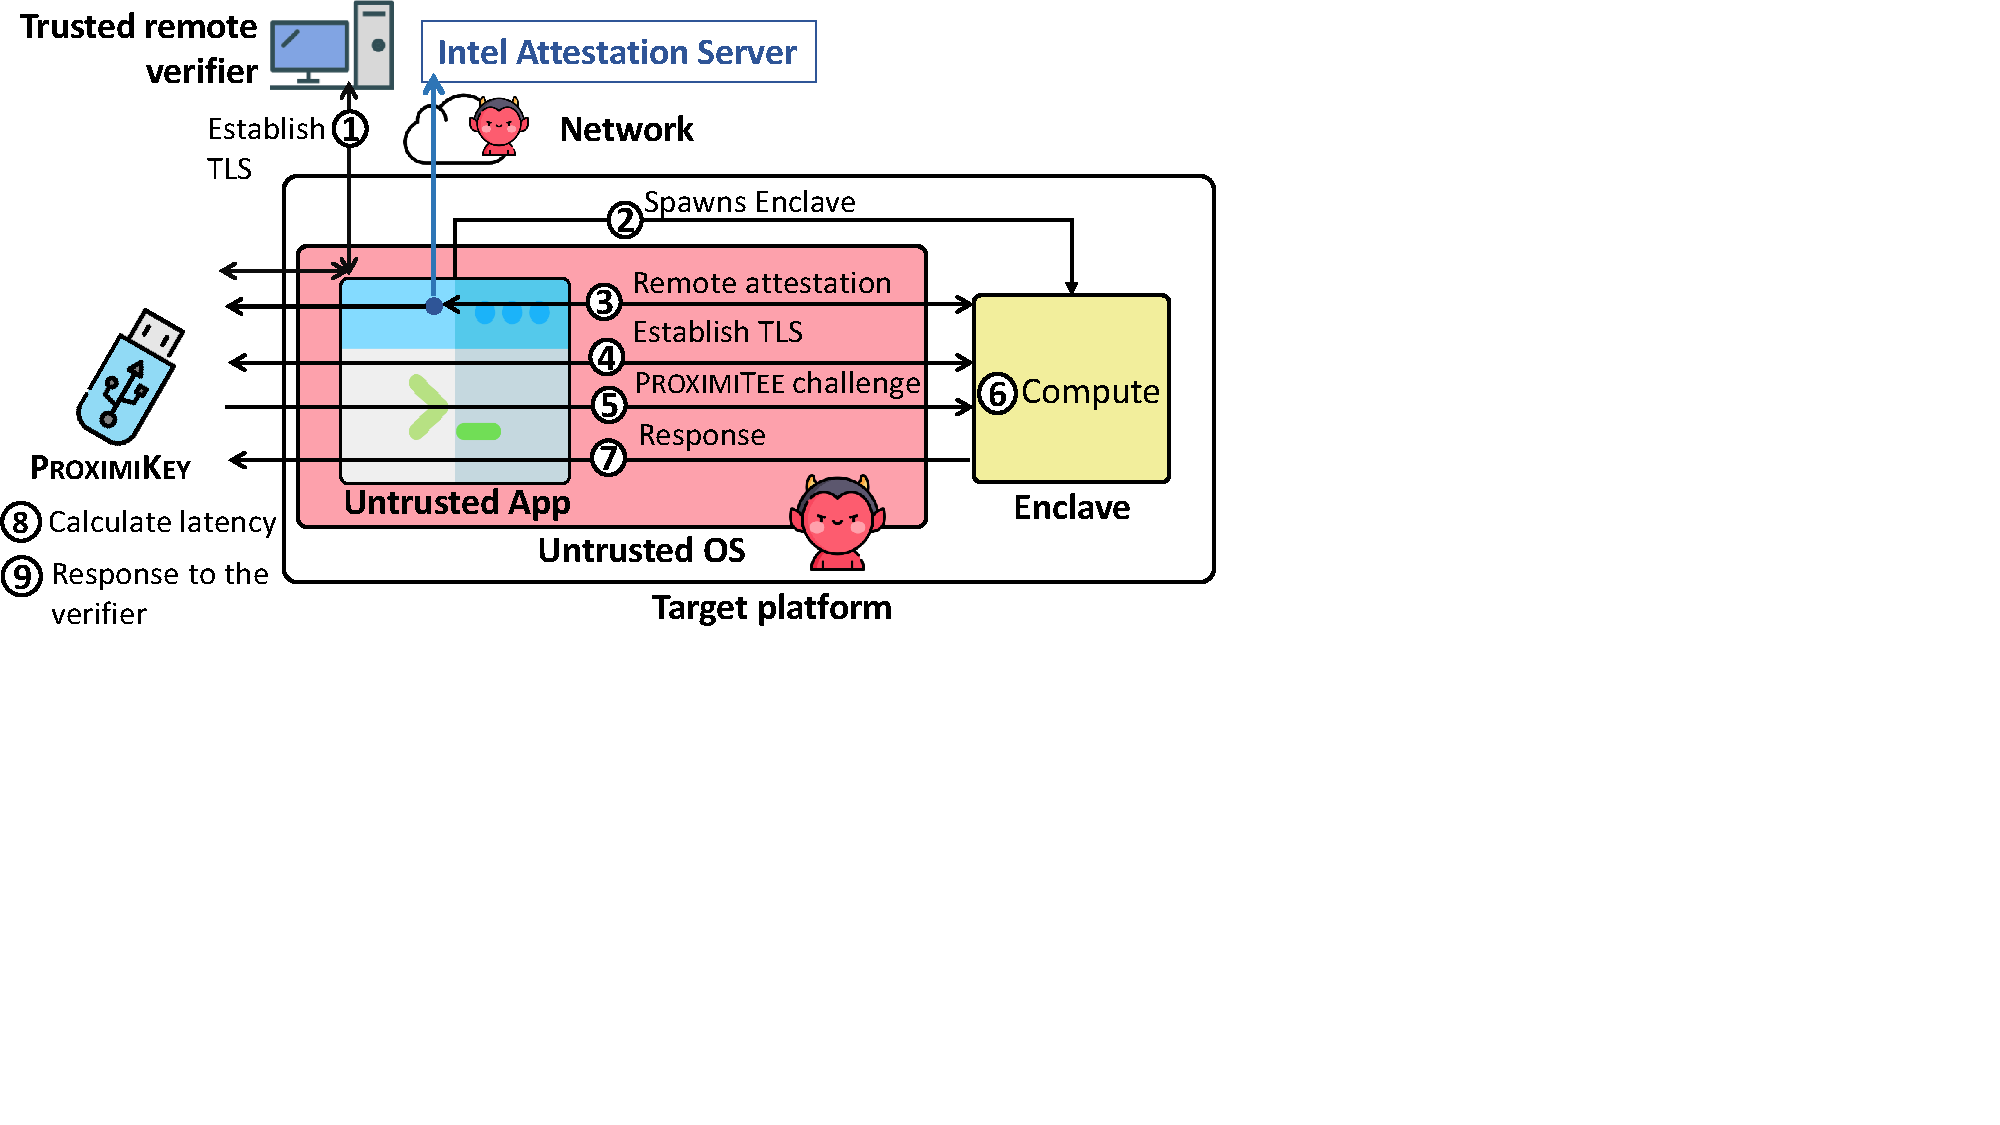
\includegraphics[trim={0 8cm 13.2cm 0},clip,width=\linewidth]{chapters/ProximiTEE/images_new/distance_bound.pdf}
 \caption[\name attestation]{\textbf{\name attestation.} The remote verifier establishes a secure channel to the \device device that first attests the enclave and then verifies its proximity.}
 	\label{fig:systemSetUp}
\end{figure}

\begin{enumerate}%
 
  \item[\one] The remote verifier establishes a secure channel (e.g., \tls) to the certified \device. An assisting but untrusted user-space application facilitates the connection on the target platform, acting as a transport channel between the remote verifier and the \device (and later also the enclave). As part of this first step, the remote verifier specifies which enclave should be executed.%

  \item[\two] The untrusted application creates and starts the attestation target enclave.%

  \item[\three] \device performs the standard remote attestation to verify the code configuration of the enclave with the help of the IAS server or using a custom DCAP procedure (see Section~\ref{ch:background:SGX:remote}). In the attestation protocol, the device learns the public key of the attested enclave.%

  \item[\four] \device establishes a secure channel (e.g., \tls) to the enclave using that public key.

  \item[\five] \device performs a distance-bounding protocol that consists of $n$ rounds, where each round is formed by steps \five to \eight.
  %(see Figure~\ref{fig:challengeResponse}).
  At the beginning of each round \device generates a random challenge $r$ and sends it to the enclave over the TLS channel.

  \item[\six] The enclave increments the received challenge by one $(r+1)$.

  \item[\seven] The enclave sends a response ($r+1$) back to the \device over the \tls channel.

  \item[\eight] \device verifies that the response value is as expected (i.e., $r+1$) and checks if the latency of the response is below a threshold (\connect). Successful proximity verification requires that the latency is below the threshold for at least $k \times n$ responses, where $k \in (0, 1]$ is a percentage of the total number of responses $n$.

  \item[\nine] If proximity verification is successful, the \device notifies the remote verifier over the \tls channel (constructed in step \one). The verifier starts using the \device TLS channel to send messages to the enclave.
\end{enumerate}


\myparagraph{Periodic proximity verification} 

After the initial connection establishment, the \device device performs \emph{periodic} proximity verification on the attested enclave. \device sends a new random challenge $r$ at frequency $f$, verifies the correctness of the received response, and measures its latency. The latest $w$ latencies are stored in a sliding window data structure, as shown in Figure~\ref{fig:slidingWindow}.

\begin{figure}[t]
  \centering
   %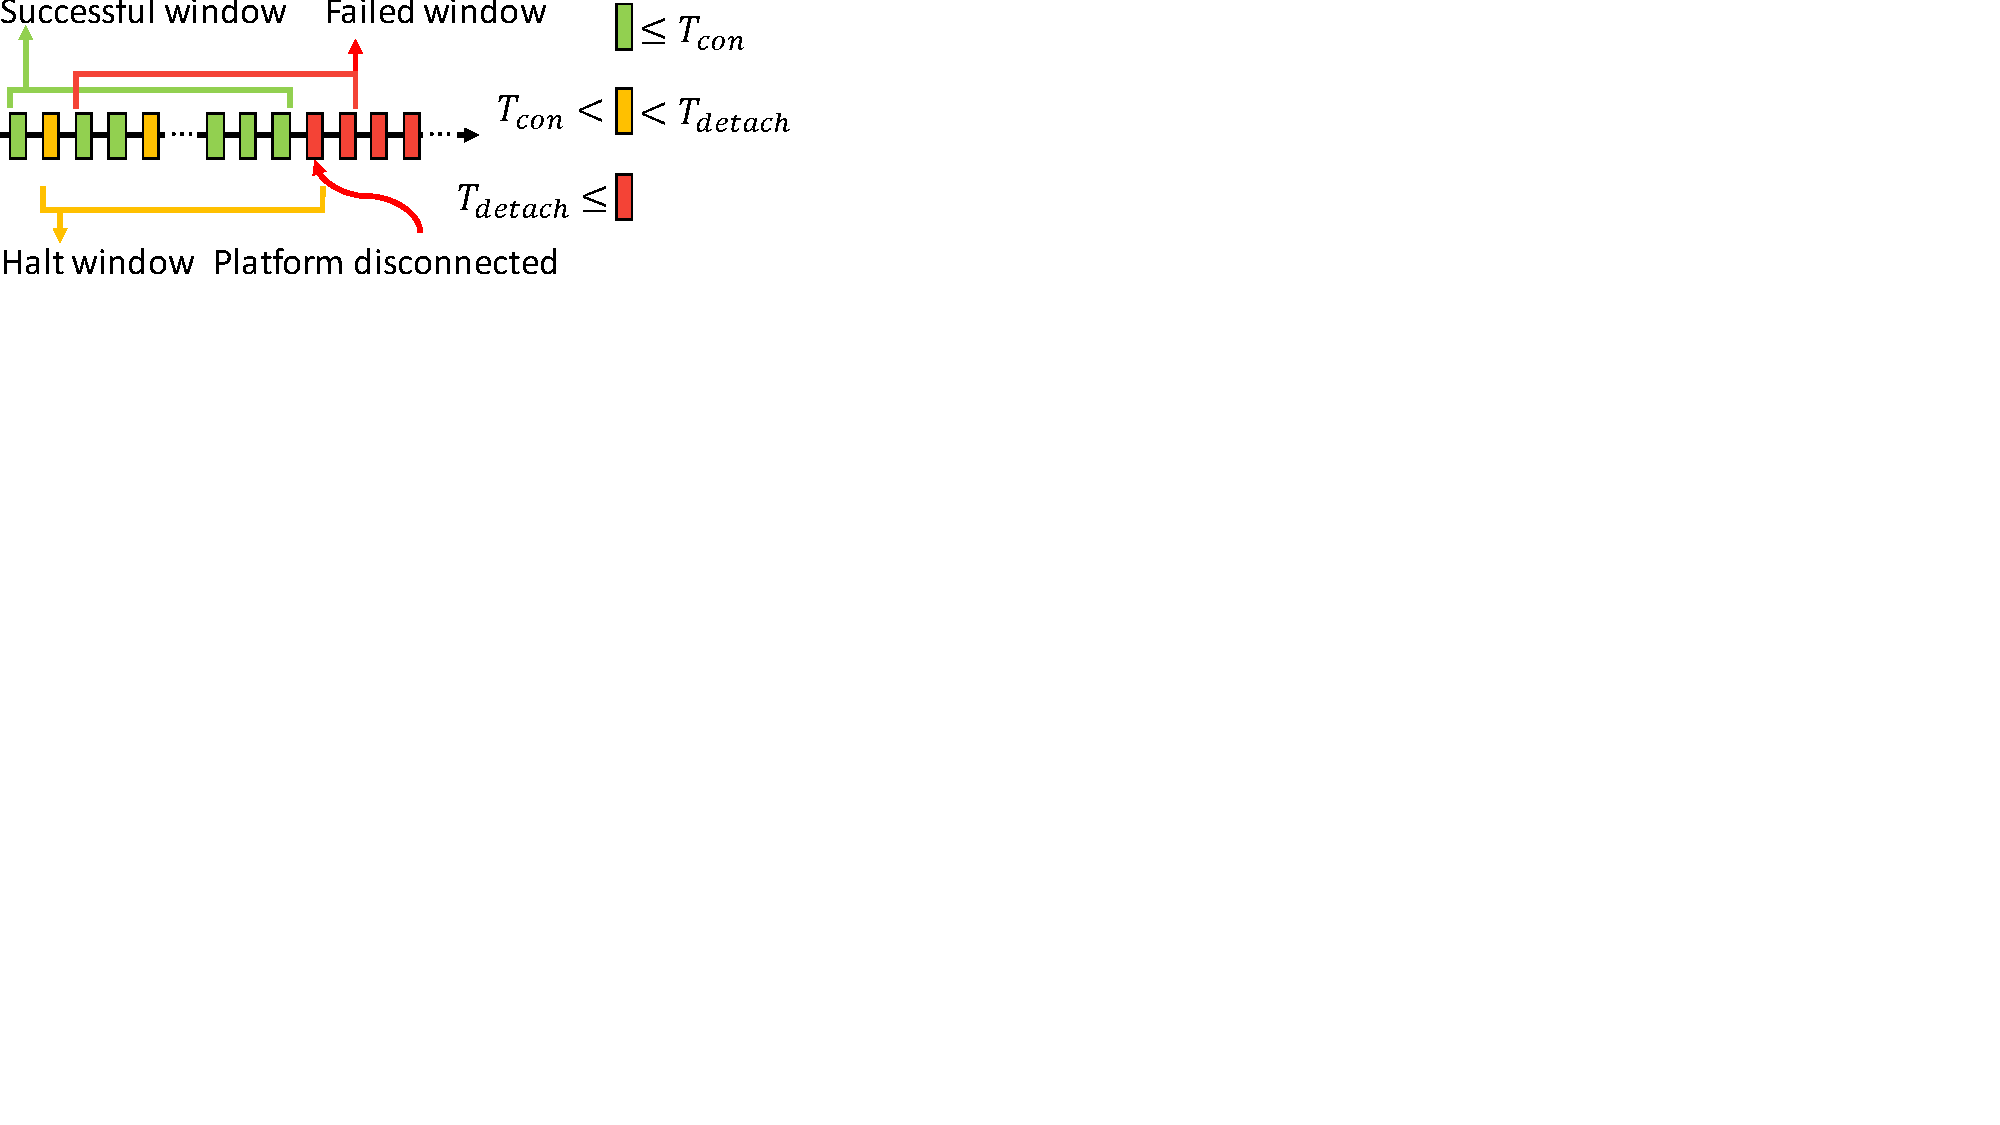
\includegraphics[trim={0 14cm 20cm 0}, clip, width=0.7\linewidth]{chapters/ProximiTEE/figures/SlidingWindow_1.pdf}
   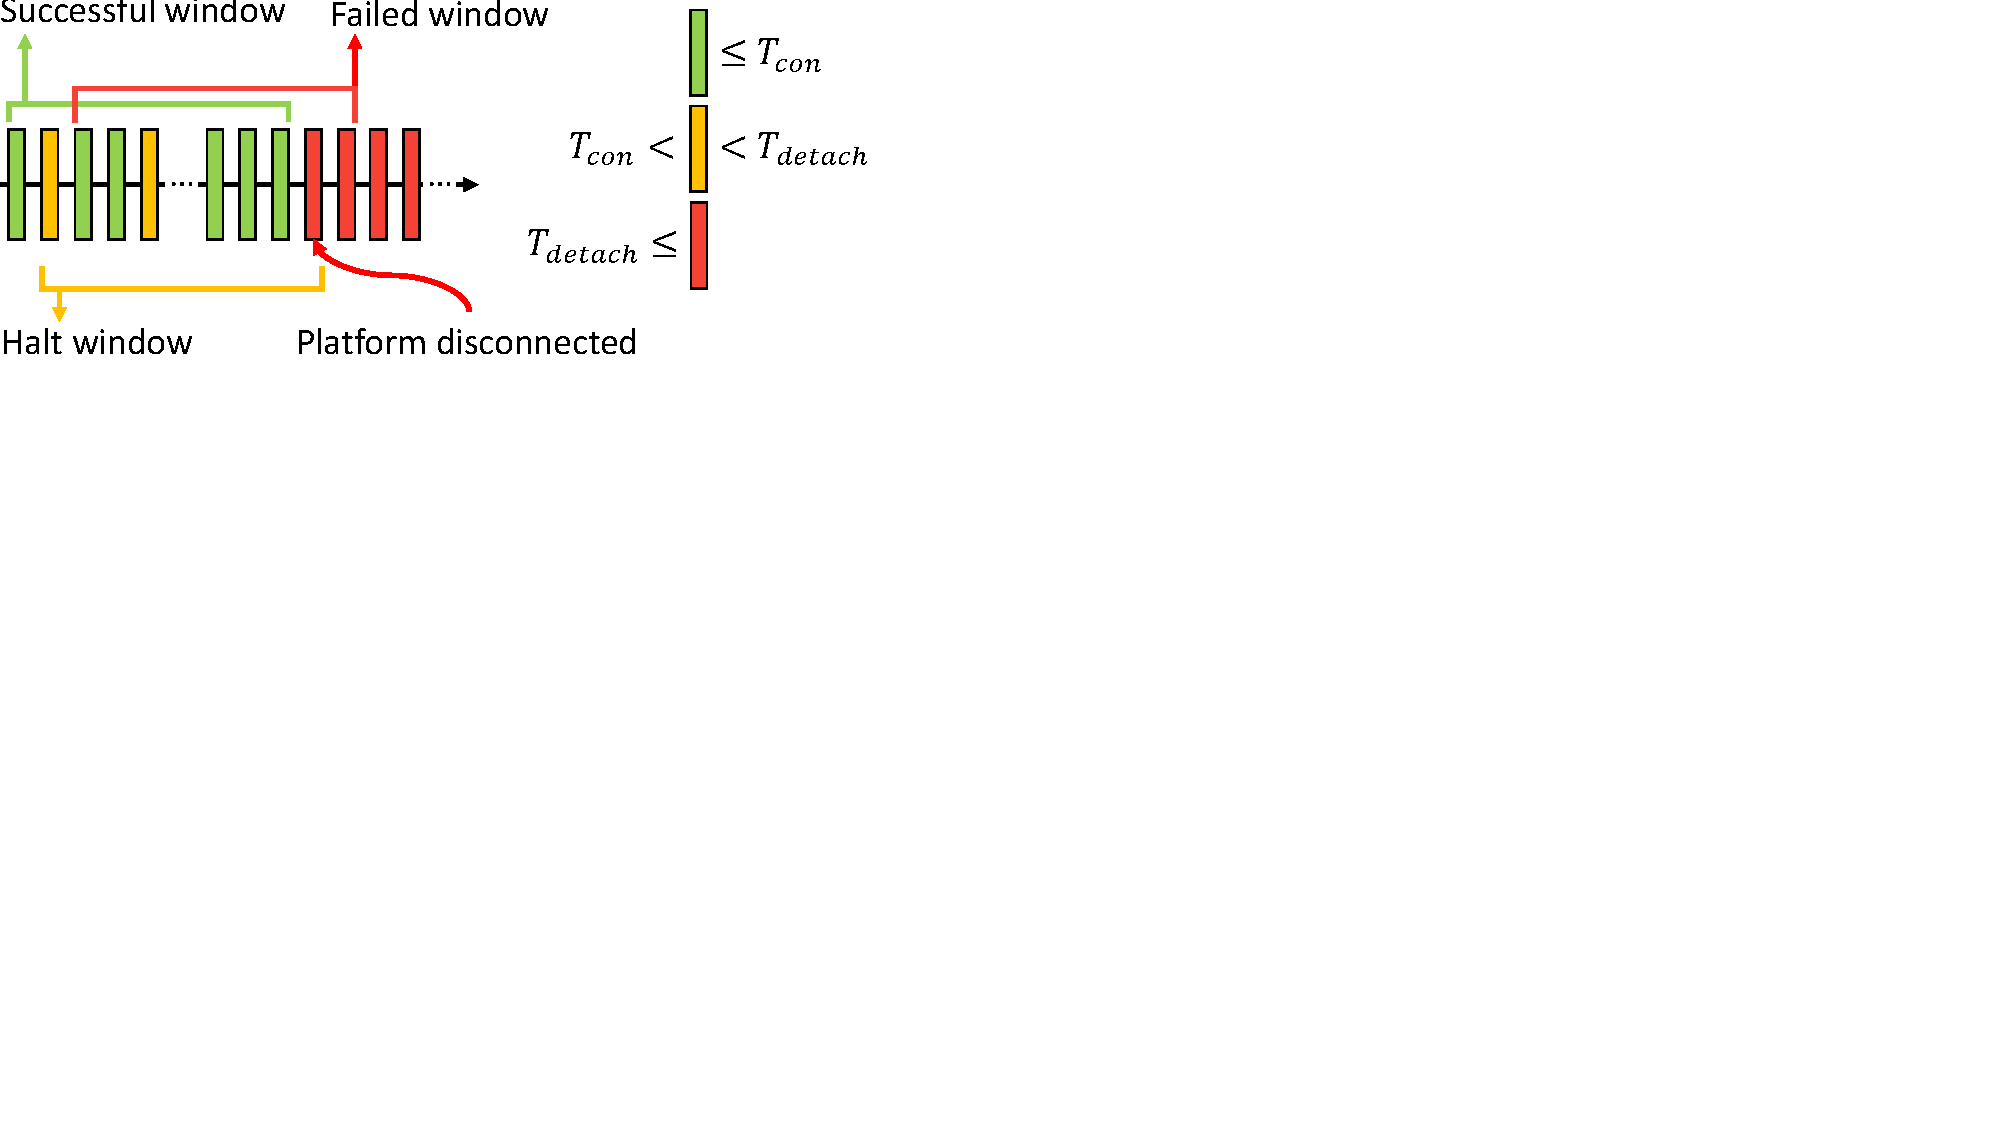
\includegraphics[trim={0 12.5cm 19cm 0}, clip, width=0.7\linewidth]{chapters/ProximiTEE/figures/SlidingWindow.pdf}
    \caption[\name periodic proximity verification]{\textbf{Sliding window} for periodic proximity verification with three different types of challenge-response latencies.}
    \label{fig:slidingWindow}
\end{figure}

As elaborated in Section~\ref{sec:evaluation}, there are three types of latencies in the presence of relay attacks. The first type of response is received faster than the threshold \connect (green in Figure~\ref{fig:slidingWindow}). These responses can only be produced if no attack is taking place. In the second type of response, the latency exceeds \connect, but it is below another, higher threshold \detach (yellow); these are sometimes observed during legitimate connections and sometimes during relay attacks. And third, the latency is equal to or exceeds \detach (red); these latencies are only observed while a relay attack is being performed. Given such a sliding window of periodic challenge-response latencies, we define the following rules for halting or terminating the connection:

\begin{enumerate}
  \item \emph{Successful window: no action.} If at least $k$ responses have latency $\leq$\connect and none of the responses has latency$\geq$\detach, the current window legitimate, and \device keeps the connection active.
 
  \item \emph{Halt window: prevent communication.} If one of the responses has latency $\geq$\detach, we consider the current window a ``halt window,'' and \device stops forwarding data to the enclave until the current window is legitimate again.

  \item \emph{Failed window: terminate channel.} If two or more responses have latencies $\geq$\detach, we consider the current window a ``failed window'', and \device terminates the communication and thus revokes the attested platform.
\end{enumerate}